\documentclass[10pt]{beamer}

\usepackage{../macros}
\title{Jeu de roulette}

\hypersetup{
  pdftitle =  {Jeu de roulette}
}

\begin{document}

\maketitle



%%%%%%%%%%%%%%%%%%%%%%%%%%%%%%%%%%%%%%%%%%%%%%%%%%%%%%%
\begin{frame}
  \frametitle{Roulette (jeu de hasard)}
  
  La roulette fait son apparition en Italie au début du XVIIe siècle. \\
  Ce jeu est surtout joué dans les casinos.
  
  \begin{columns}[c]
    \begin{column}{0.58\textwidth}
      \begin{itemize}
      \item La roulette est un jeu de hasard dans lequel chaque joueur, assis autour d'une table de jeu, mise sur un ou plusieurs numéros, une couleur \dots 
      \item Le tirage du numéro s'effectue à l'aide d'une bille jetée dans un récipient circulaire tournant et muni d'encoches ayant des numéros de différentes couleurs.
      \item Pour la roulette anglaise et française, 37 cases numérotées de 0 à 36 alternativement rouges et noires, à l'exception du zéro, vert.
    \end{itemize}
  \end{column}
  \begin{column}{0.42\textwidth}
    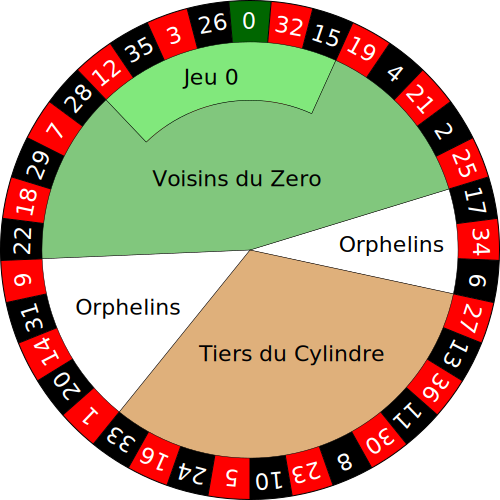
\includegraphics[width=0.95\textwidth]{european_roulette_wheel}
    \\
    \footnotesize{La description et les images sont tirées de \href{https://fr.wikipedia.org/wiki/Roulette_(jeu_de_hasard)}{Wikipedia}.}
  \end{column}
\end{columns}

\end{frame}





%%%%%%%%%%%%%%%%%%%%%%%%%%%%%%%%%%%%%%%%%%%%%%%%%%%%%%%
\begin{frame}
  \frametitle{Miser à la roulette}
  Nous utiliserons seulement une partie des mises de la roulette.
  
  \begin{columns}[c]
    \begin{column}{0.53\textwidth}
      \begin{tabular}{lcc}
        \toprule
        \textbf{Mise}         & \textbf{\#num} & \textbf{Gain} \\
        \midrule
        \textbf{Plein}        & 1                  & $\times$ 35   \\
        \textbf{Transversale} & 3                  & $\times$ 11   \\
        1-3, 4-6, 7-9, \dots                                      \\
        \textbf{Colonne}      & 12                 & $\times$ 2    \\
        1-34, 2-35, 3-36                                           \\
        \textbf{Douzaine}     & 12                 & $\times$ 2    \\
        1-12, 13-24, 25-36                                         \\
        \textbf{Pair-Impair}  & 18                 & $\times$ 1    \\
        \textbf{Manque-Passe} & 18                 & $\times$ 1    \\
        1-18, 19-36                                                \\
        \bottomrule
      \end{tabular}
      \begin{block}{Question}
        Quel est le rôle du numero 0 ?
      \end{block}
    \end{column}
    \begin{column}{0.47\textwidth}
      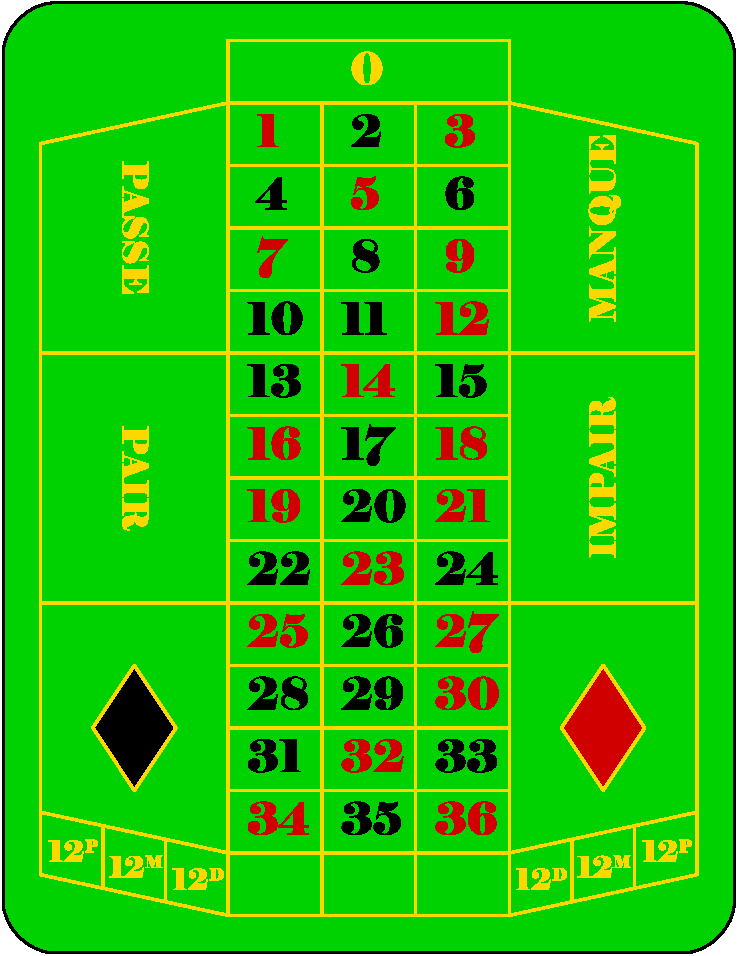
\includegraphics[width=0.99\textwidth]{roulette_french}
    \end{column}
  \end{columns}

\end{frame}


%%%%%%%%%%%%%%%%%%%%%%%%%%%%%%%%%%%%%%%%%%%%%%%%%%%%%%%
\begin{frame}
  \frametitle{Programmer un jeu de roulette en mode solo}
  \begin{alertblock}{Moteur du jeu}
    \begin{enumerate}
    \item L'utilisateur saisit sa mise.
    \item Le croupier tire le numéro gagnant au hasard. 
    \item Le croupier détermine le gain et le renvoie au joueur.
    \end{enumerate}
  \end{alertblock}


  \begin{block}{Questions}
    \begin{itemize}
    \item Comment représenter la mise du joueur ?
    \item Comment intéragir avec le joueur ?
    \item Comment tirer le numéro gagnant ? 
    \item Comment calculer facilement le gain du joueur ?
    \end{itemize}
  \end{block}
\end{frame}



%%%%%%%%%%%%%%%%%%%%%%%%%%%%%%%%%%%%%%%%%%%%%%%%%%%%%%%
\begin{frame}
  \frametitle{Représenter la mise du joueur}
  \begin{description}[Montant]
  \item[Type] un nombre identifie le type de la mise (plein, transversale \dots).
  \item[Numéro] un numéro gagnant de la mise. Remarquez que pour chaque type de myse, un numéro n'apparaît que dans une seule combinaison gagnante.
  \item[Montant] le montant en de la mise.
  \end{description}

  
\begin{columns}[c]
\begin{column}{0.58\textwidth}
  \begin{exampleblock}{Exemples de mise}
  \end{exampleblock}
  \begin{tabular}{lll}
    \toprule
    Type & Num & Mise             \\
    \midrule
    1    & 1   & Plein sur le 1   \\
    2    & 8   & Transversale 7-9 \\
    3    & 8   & Colonne 2-35     \\
    4    & 18  & Douzaine 13-24   \\
    5    & 8   & Pair             \\
    6    & 8   & Manque           \\
    \bottomrule
  \end{tabular}
  \begin{alertblock}{Pas d'unicité !}
    Manque avec le type 6 et n'importe quel numéro entre 1 et 18.
  \end{alertblock}
  \end{column}
\begin{column}{0.42\textwidth}
    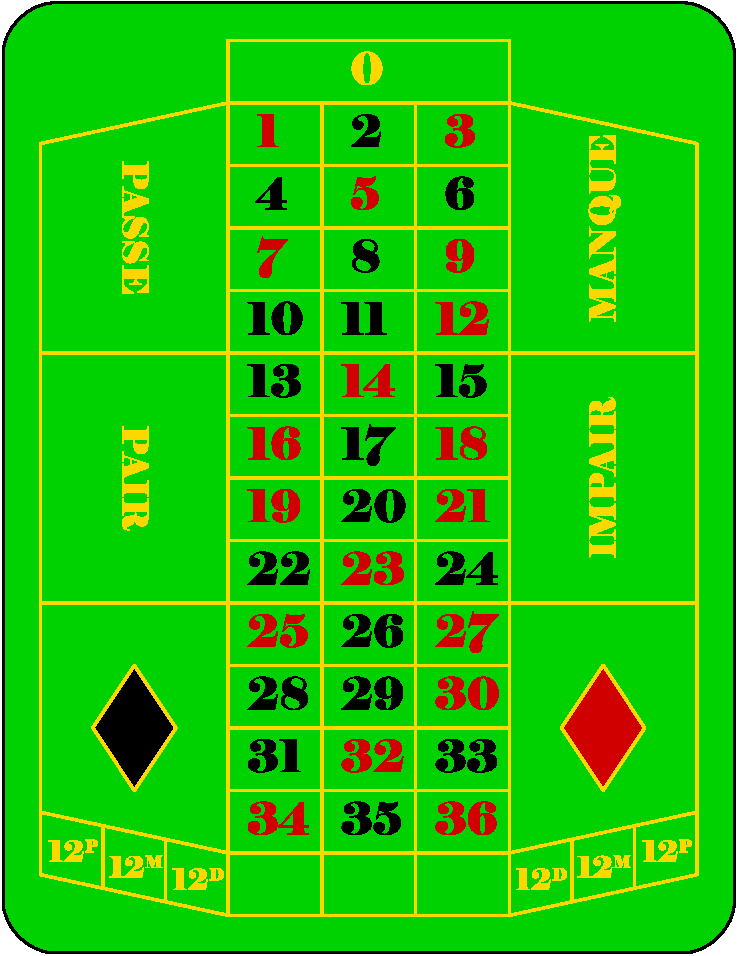
\includegraphics[width=0.99\textwidth]{roulette_french}
  \end{column}
\end{columns}

\end{frame}


%%%%%%%%%%%%%%%%%%%%%%%%%%%%%%%%%%%%%%%%%%%%%%%%%%%%%%%
\begin{frame}[fragile]
  \frametitle{Moteur de jeu}
  \lstinputlisting[linerange=67-85]{roulette.R}
\end{frame}

%%%%%%%%%%%%%%%%%%%%%%%%%%%%%%%%%%%%%%%%%%%%%%%%%%%%%%%
\begin{frame}[fragile]
  \frametitle{Saisir le type de la mise}
  \lstinputlisting[style=editor,linerange=1-7]{roulette.R}
  \begin{lstlisting}
> LireMise()
Veuillez saisir le type de la mise :  

1: Plein
2: Transversale
3: Colonne
4: Douzaine
5: Pair-Impair
6: Manque-Passe

Selection: 2
[1] 2    
\end{lstlisting}

\end{frame}

%%%%%%%%%%%%%%%%%%%%%%%%%%%%%%%%%%%%%%%%%%%%%%%%%%%%%%%
\begin{frame}[fragile]
  \frametitle{Saisir le numéro gagnant de la mise}  
  \begin{description}
  \item[\texttt{cat}] afficher un message dans l'interpréteur
  \item[\texttt{scan}] lire un nombre dans l'interpréteur
  \item[\texttt{stopifnot}] arréter le programme si une condition n'est pas satisfaite
  \end{description}
  \lstinputlisting[style=editor,linerange=8-13]{roulette.R}

  \begin{lstlisting}
> LireNumero()
Veuillez saisir un numéro de la mise :
1: 10
[1] 10
>  LireNumero()
Veuillez saisir un numéro de la mise :
1: 38
Error in LireNumero() : numero <= 36 is not TRUE      
\end{lstlisting}
\end{frame}


%%%%%%%%%%%%%%%%%%%%%%%%%%%%%%%%%%%%%%%%%%%%%%%%%%%%%%%
\begin{frame}[fragile]
  \frametitle{Saisir le montant de la mise}
  Un peu répétitif ! On modifie légérement la fonction précédente.
  \lstinputlisting[style=editor,linerange=15-20]{roulette.R}
\end{frame}


%%%%%%%%%%%%%%%%%%%%%%%%%%%%%%%%%%%%%%%%%%%%%%%%%%%%%%%
\begin{frame}[fragile]
  \frametitle{Tirer le numéro gagnant au hasard}
    La \href{https://fr.wikipedia.org/wiki/Simulation_informatique}{simulation informatique} désigne l'exécution d'un programme informatique sur un ordinateur ou un réseau en vue de simuler un phénomène physique réel et complexe (par exemple : chute d’un corps sur un support mou, résistance d’une plateforme pétrolière à la houle, \dots).

    \begin{block}{Simuler le tirage du numéro gagnant}
      Générer un entier \alert{pseudo-aléaloire} compris entre 0 et 36.
    \end{block}
    \lstinputlisting[style=editor,linerange=22-24]{roulette.R}
    \begin{lstlisting}
> TirerNumeroGagnant()
[1] 13
> TirerNumeroGagnant()
[1] 2
\end{lstlisting}
\end{frame}


%%%%%%%%%%%%%%%%%%%%%%%%%%%%%%%%%%%%%%%%%%%%%%%%%%%%%%%
\begin{frame}[fragile]
  \frametitle{Déterminer le gain en fonction de la mise et du tirage}
  Pour écrire des programmes corrects, il faut les structurer.
  \lstinputlisting[style=editor,linerange=56-64]{roulette.R}
  \begin{itemize}
  \item Ici, c'est un peu répétitif et fastidieux \dots
  \item On peut utiliser d'autres paradigmes ou techniques pour l'eviter.
  \end{itemize}

\end{frame}

%%%%%%%%%%%%%%%%%%%%%%%%%%%%%%%%%%%%%%%%%%%%%%%%%%%%%%%
\begin{frame}[fragile]
  \frametitle{Déterminer le gain I}
  \lstinputlisting[style=editor,linerange=26-39]{roulette.R}

  
\begin{columns}[t]
\begin{column}{0.48\textwidth}
  \begin{lstlisting}
> GainTransversale(3, 1)
[1] 11
> GainTransversale(3, 6)
[1] 0
\end{lstlisting}
\end{column}
\begin{column}{0.48\textwidth}
  \begin{lstlisting}
> GainColonne(3, 1)
[1] 0
> GainColonne(3, 6)
[1] 2
  \end{lstlisting}
\end{column}
\end{columns}
\end{frame}
%%%%%%%%%%%%%%%%%%%%%%%%%%%%%%%%%%%%%%%%%%%%%%%%%%%%%%%
\begin{frame}[fragile]
  \frametitle{Déterminer le gain II}
  \begin{exampleblock}{À vous de jouer !}
    \lstinputlisting[style=edblock,linerange=61-63]{roulette.R}
  \end{exampleblock}
  \begin{lstlisting}
> GainDouzaine(1, 11)
[1] 2
> GainDouzaine(1, 16)
[1] 0
> GainManquePasse(1, 19)
[1] 0
> GainManquePasse(21, 19)
[1] 1
> GainPairImpair(1, 11)
[1] 1
> GainPairImpair(1, 16)
[1] 0
  \end{lstlisting}
\end{frame}

%%%%%%%%%%%%%%%%%%%%%%%%%%%%%%%%%%%%%%%%%%%%%%%%%%%%%%%
\begin{frame}[fragile]
  \frametitle{Exécution du programme}
  \begin{lstlisting}
> JouerRoulette()
Veuillez saisir le type de la mise :  

1: Plein
2: Transversale
3: Colonne
4: Douzaine
5: Pair-Impair
6: Manque-Passe

Selection: 1
Veuillez saisir un numéro gagnant de la mise :
1: 0
Veuillez saisir le montant de la mise :
1: 0
Le numéro gagnant est le 34.
Vous avez gagné 0.
[1] 0
\end{lstlisting}

\end{frame}


%%%%%%%%%%%%%%%%%%%%%%%%%%%%%%%%%%%%%%%%%%%%%%%%%%%%%%%



%%%%%%%%%%%%%%%%%%%%%%%%%%%%%%%%%%%%%%%%%%%%%%%%%%%%%%%
 \questionSlide

%%%%%%%%%%%%%%%%%%%%%%%%%%%%%%%%%%%%%%%%%%%%%%%%%%%%%%%
 \appendix
 \backupSlides
%%%%%%%%%%%%%%%%%%%%%%%%%%%%%%%%%%%%%%%%%%%%%%%%%%%%%%%



%%%%%%%%%%%%%%%%%%%%%%%%%%%%%%%%%%%%%%%%%%%%%%%%%%%%%%%
% \begin{frame}[allowframebreaks]{References}

%   % \bibliography{../bib_parallelism,../bib_others}
%   % \bibliographystyle{abbrv}

% \end{frame}

\end{document}

%%% Local Variables:
%%% mode: latex
%%% TeX-master: t
%%% End:
